\documentclass[pdflatex,compress]{beamer}

%\usetheme[dark,framenumber,totalframenumber]{ElektroITK}
\usetheme[darktitle,framenumber,totalframenumber]{ElektroITK}

\usepackage{graphicx}

\title{METODE NUMERIK}
\subtitle{Deret Taylor dan Analisis Galat}

\author{Tim Dosen Pengampu}

\begin{document}
	
% ----------------------------------------------------------------------------
% *** Titlepage <<<
% ----------------------------------------------------------------------------
\maketitle
% ----------------------------------------------------------------------------
% *** END of Titlepage >>>
% ----------------------------------------------------------------------------
\section{Deret Taylor}

\begin{frame}
	\frametitle{Deret Taylor}
	\begin{itemize}
		\item Kakas (\textit{tools}) yang sangat penting dalam metode numerik adalah \textbf{deret Taylor}.
		\item Deret Taylor adalah kakas yang utama untuk menurunkan suatu metode numerik.
		\item Deret Taylor berguna untuk menghampiri fungsi ke dalam bentuk polinom
		\item Fungsi yang rumit menjadi sederhana dengan deret Taylor
	\end{itemize}
\end{frame}

\begin{frame}
	\frametitle{Definisi Deret Taylor}
	\begin{itemize}
		\item Andaikan $ f $ dan semua turunannya, $ f' $, $ f'' $, $ f''' $, ..., menerus di dalam selang $ [a, b] $. Misalkan $ x_0 \subset [a, b] $, maka untuk nilai-nilai $ x $ di sekitar $ x_0 $ (Gambar 2.1) dan $ x \subset [a, b] $, $ f(x) $ dapat diperluas (diekspansi) ke dalam deret Taylor:
		\begin{align*}
			f(x) =& f(x_0) + \frac{(x-x_0)}{1!}f'(x_0) + \frac{(x-x_0)^2}{2!}f''(x_0) \\
			&+ \frac{(x-x_0)^3}{1!}f'''(x_0) + \cdots + \frac{(x-x_0)^m}{m!}f^m(x_0) + \cdots
		\end{align*}
		\begin{center}
			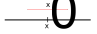
\includegraphics[width=0.5\linewidth]{img/img101}
		\end{center}
	\end{itemize}
\end{frame}

\begin{frame}
	\frametitle{Definisi Deret Taylor}
	\begin{itemize}
		\item Misalkan $ x - x_0 = h $, maka:
		\begin{align*}
			f(x) =& f(x_0) + \frac{h}{1!}f'(x_0) + \frac{h^2}{2!}f''(x_0) + \frac{h^3}{1!}f'''(x_0) \\
			&+ \cdots + \frac{h^m}{m!}f^m(x_0) + \cdots
		\end{align*}
	\end{itemize}
\end{frame}

\begin{frame}
	\frametitle{Contoh 1}
	Hampiri fungsi $ f(x) = \sin(x) $ ke dalam deret Taylor di sekitar $ x_0 = 1 $. \\
	Penyelesaian: \\
	
	\begin{align*}
		f(x) = \sin(x)
	\end{align*}
	
	
\end{frame}
% ----------------------------------------------------------------------------
	
\end{document}
